\documentclass[letterpaper, reqno,11pt]{article}
\usepackage[margin=1.0in]{geometry}
\usepackage{color,latexsym,amsmath,amssymb,graphicx, float}
\usepackage{hyperref}

\hypersetup{
colorlinks=true,
linkcolor=magenta,
filecolor=magenta,
urlcolor=cyan,
}

\graphicspath{ {images/} }

\newcommand{\RR}{\mathbb{R}}
\newcommand{\CC}{\mathbb{C}}
\newcommand{\ZZ}{\mathbb{Z}}
\newcommand{\QQ}{\mathbb{Q}}
\newcommand{\NN}{\mathbb{N}}
\newcommand{\st}{\text{ s.t.}\ }
\newcommand{\ep}{\epsilon}

\begin{document}
\pagenumbering{arabic}
\title{PHYS 301 Homework 4}
\date{November 01, 2021}
\author{Xander Naumenko}
\maketitle

{\noindent\bf Question 1.} Note that the charge density in spherical coordinates is $\delta(r-R)$ for the upper section and $-\delta(r-R)$ for the lower section. Setting up the integral for the electric dipole we then get 

\begin{align*}
    \vec p&=\int\vec r^\prime \rho(\vec r^\prime)d\tau^\prime=\int_0^\infty\int_0^{\pi}\int_0^{2\pi}r\rho(\vec r)r^2\sin\theta\begin{pmatrix}\sin\theta\cos\phi\\\sin\theta\sin\phi\\\cos\theta\end{pmatrix} d\phi d\theta dr\\
    &=2\pi\int_0^{\pi/2}\sigma R^3\sin\theta\cos\theta \hat zd\theta-2\pi\int_{\pi/2}^\pi\sigma R^3\sin\theta\cos\theta \hat zd\theta\\
    &=4\pi R^3\sigma\hat z\int_0^{\pi/2}\sin\theta\cos\theta d\theta=4\pi R^3\sigma (\frac12 u^2)\bigg|_{0}^1=2\pi R^3\sigma\hat z
\end{align*}

As can be seen the x and y components go to zero when you integrate over $\phi$, leaving just a $z$ component. 

{\noindent\bf Question 2a.} 

\[
    \sigma_{bound, outer}=\vec P\cdot \hat n =\frac{k\hat s}{a^2}\cdot \hat s=\frac k{a^2}   
\]

\[
    \sigma_{bound, inner}=\vec P\cdot \hat n =-\frac{k\hat s}{b^2}\cdot \hat s=-\frac k{b^2}   
\]

\[
    \rho_{bound}=-\nabla\cdot\vec P=-\nabla\cdot \frac{k\hat s}{s^2}=-\frac1s(\frac{d}{ds}(\frac ks))=\frac k{s^3}
\]

{\noindent\bf Question 2b.} To find $\vec E$, we use a gaussian cylinder of radius $s$ and height $h$ around the center of the insulating rod. For $s<b$ there is no charge enclosed so by symmetry the $\vec E$ field is zero, For $b<s<a$, applying Gauss's law gives 

$$
    \Phi=2\pi sh E=\frac{q}{\epsilon_0}=-\frac{1}{\epsilon_0}\int_0^h\int_b^s\int_0^{2\pi}\frac{k}{r^3}r+\frac{k}{b^2}r\delta(r-b) d\phi drdz=-\frac{2\pi hk}{\epsilon_0r}\bigg|_b^s-\frac{\pi hk}{\epsilon_0 b}
$$

\[
    =-\frac{2\pi hk}{\epsilon_0s}
\]

\[
    \vec E=-\frac{k}{\epsilon_0 s^2}\hat s=-\frac1{\epsilon_0}\vec P
\]

For $s>a$, using the same gaussian cylinder we see that 

\[
    \Phi=2\pi sh E=\frac{q}{\epsilon_0}=\frac1{\epsilon_0}(-\frac{2\pi hk}{\epsilon_0a}+\int_0^h\int_b^a\int_0^{2\pi} \frac{k}{a^2}\delta(r-a)d\phi drdz)=0\implies \vec E=\vec 0
\]

As expected, this means that the electric field is nonzero only inside the polarized material. 

{\noindent\bf Question 2c.} Since $\vec D$ only depends on the free charges and there are none, $\vec D=\vec 0$ everywhere. 

{\noindent\bf Question 3a.} 

\[
    \sigma_B=\vec P\cdot \hat n=P_0\vec r\cdot \hat r=P_0a
\]

\[
    \rho_B=-\nabla \cdot \vec P=-\nabla \cdot (P_0 r)=-3P_0
\]

{\noindent\bf Question 3b.} First we find the $\vec D$ field. Since there are no free charges and $\vec D$ depends only on free charges, we can conclude that $\vec D=\vec 0$ everywhere. Since $\vec D=\vec 0=\epsilon_0\vec E+\vec P$, we have that $\vec E=-\frac1{\epsilon_0}\vec P=-\frac{P_0 }{\epsilon_0}\vec r$ for $r<a$, and $\vec E=\vec 0$ for $r>a$. A sketch of this can be seen in figure \ref{fig:3b}. Although the electric field suddently jumps accross the boundary of the edge of the sphere, this is fine as the electric field does not have to be continuous. 

\begin{figure}[htbp]
\centering
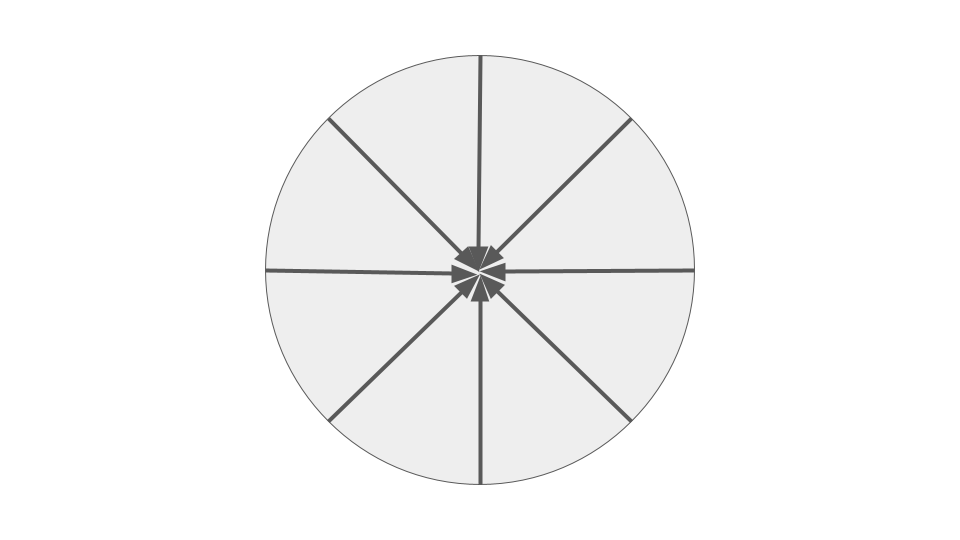
\includegraphics[width=\textwidth]{3b}
\caption{Field inside the sphere for question 3b. The electric field outside the sphere is zero, so no field lines are drawn. }
\label{fig:3b}
\end{figure}

{\noindent\bf Question 4a.} Considering a Gaussian pillbox with the bottom just below the bottom plate and the top at an point between the plates, we see that $\vec D=-\sigma\hat z$ (taking $z$ to be the positive vertical direction in the diagram), since this is the exact same situation as we hade for a conducting slab because we can ignore the bound charges for the calculation of $\vec D$. 

{\noindent\bf Question 4b.} To find $\vec E$ we will use the relationship $\vec D=\epsilon\vec E$ when considering a point within a linear dialectric (which both slabs are in this case). Thus within the upper plate, $\vec E=\frac1{\epsilon_1}\vec D=-\frac{\sigma}{\epsilon_1}\hat z$ and the electric field inside the bottom slab is $\vec E=-\frac{\sigma}{\epsilon_2}\hat z$. 

{\noindent\bf Question 4c.} For a linear dialectric it is true that $\vec P=\epsilon_0(\epsilon_r - 1)\vec E$. We also have that $\sigma_B=\vec P\cdot\hat n$. Combining these two facts gives that for the top surface, 

\[
    \sigma_{B1}=-(\epsilon_1-\ep_0)\frac{\sigma}{\epsilon_1}\hat z\hat n=-\sigma(1-\frac{\ep_0}{\epsilon_1})
\]

Similarly for the bottommost surface: 

\[
    \sigma_{B2}=\sigma(1-\frac{\ep_0}{\epsilon_2})
\]

For the middle section, it is the sum of the two individual surface charge densities. Note however that since we're looking at the opposite side of each slab as calculated for above the signs are reversed. 

$$
    \sigma_{B(1+2)}=-(\sigma_{B1}+\sigma_{B2})=\sigma\ep_0(\frac1{\epsilon_2}-\frac1{\epsilon_1})
$$

{\noindent\bf Question 4d.} First we find the voltage. Since $V=-\int\vec E\dot dl$, all we have to do is integrate over the two dialectrics with the electric field found above. Also the electric field in the dialectrics is constant, so this simply gives $V=\frac{\sigma d}{2\epsilon_0}(\frac1{\epsilon_1}+\frac1{\epsilon_2})$. Then using the definition of capacitance $C=\frac{Q}{V}$, we get 

$$
    C=\frac QV=\frac{\sigma L^2}{\frac{\sigma d}{2}(\frac1{\epsilon_1}+\frac1{\epsilon_2})}=\frac{2L^2}{d(\frac1{\epsilon_1}+\frac1{\epsilon_2})}=\frac{2L^2\epsilon_1\epsilon_2}{d(\epsilon_1+\ep_2)}
$$

{\noindent\bf Question 4e.} This can be verified for any location inside the capacitor. Since the question doesn't specify where to verify the laws it will be shown for a gaussian pillbox with the upper face inside the upper plate conductor and the bottom face inside the upper dialectric. 

\[
    \int_S\vec D\cdot dA=\sigma L^2=Q_f
\]

This isn't suprising given we used this property to compute $D$ originally, but it is good to confirm. For the second property: 

$$
    \int_S \vec E\cdot d\vec A=\int_S-\frac{\sigma}{\epsilon_0\epsilon_1}d\vec A=\frac{\sigma L^2}{\epsilon_0\epsilon_1}=\frac{\sigma L^2}{\epsilon_0}+\frac{\sigma_{B1} L^2}{\epsilon_0}=\frac{Q}{\epsilon_0}
$$

{\noindent\bf Question 5a.} For $r<a$ there is no charge enclosed (bound or free) so by considering a Gaussian sphere of radius $r<a$, $\vec D=\vec 0$ and $\vec E=\vec 0$. Also there is no dialectric inside so $\vec P=0$ for $r<a$ as well.

For $r>b$, again the total charge enclosed by a guassian sphere of radius $r$ is zero so $\vec D=0$ and $\vec E=0$. Also there is no dialectric so $\vec P=0$ outside as well.

For $a<r<b$, we know that the electric field must be the same in both sections of the sphere. This is because both the inside and outside are conductors, so to keep the voltage between the two surfaces consistent, the electric field must be oriented radially with no $\theta$ or $\phi$ dependence. Applying Gauss's law to the $\vec D$ field for a sphere of radius $r$, this gives 

\[
    4\pi r^2 D=2\pi r^2(\ep_0 E + \ep E)=Q\implies \vec E=\frac{Q}{2\pi r^2 (\epsilon_0+\epsilon)}\hat r
\]

\[
    \vec D=\frac{Q}{2\pi r^2}\hat r
\]

{\noindent\bf Question 5b.} Since the electric field is the same on both sides, the total charge must be distributed evenly. First, the bound charge on the dialectric side must be 

\[
    \sigma_B=\vec P\cdot\hat n=-(\epsilon-\epsilon_0)\vec E\cdot\hat r=-\frac{Q(\epsilon-\epsilon_0)}{2\pi a^2(\epsilon+\ep_0)}
\]

Since the total charge must be distributed equally, this means that $Q_{upper}=Q_{lower}+\sigma_B$ and $Q_{upper}+Q_{lower}=Q$. Then 

\[
    2\sigma_{upper}=\frac Q{2\pi a^2}+\sigma_B=\frac Q{2\pi a^2}-\frac{Q(\epsilon-\epsilon_0)}{2\pi a^2(\epsilon+\ep_0)}
\]

\[
    \sigma_{upper}=\frac{Q\epsilon_0}{2\pi a^2(\epsilon+\ep_0)}
\]

Doing the exact same calculation except for the bottom shell gives 

\[
    \sigma_{lower} = \frac{Q\epsilon}{2\pi a^2(\epsilon+\epsilon_0)}    
\]

{\noindent\bf Question 5c.} $\sigma_{B,a}$ was already determined in the previous question to be $\sigma_{B,a}=-\frac{Q(\ep-\ep_0}{2\pi a^2(\ep+\ep_0)}$. The upper section, using the exact same argument as used in part b, will be 

\[
    \sigma_{B,b}=\frac{Q}{\ep-\ep_0}{2\pi b^2(\ep+\ep_0)}    
\]

{\noindent\bf Question 5d.} To find capacitance we must find the voltage. This is the same for both sections since the electric field is the same for both. This gives:  

\[
    V=-\int \vec E\cdot \vec {dl}=\int_a^b\frac{Q}{2\pi r^2(\ep_0+\ep)}dr=\frac Q{2\pi(\ep_0+\ep)}(\frac1a-\frac1b)
\]

We can the find the total capacitance: 

\[
    C=\frac QV=2\pi(\ep_0+\ep)\frac1{\frac1a-\frac1b}=\frac{2\pi(\ep_0+\ep)ab}{b-a}
\]


{\noindent\bf Question 6a.} Due to the polarization a surface charge develops. Note that a volume charge density does not develop since in this case $\nabla\cdot \vec P=0$. Then the surface charge for the top of the cylinder is 

$$
    \sigma_{bound}=\vec P\cdot \hat n=P
$$

For the bottom a similar computation gives $\sigma_{bound}=-P$. Since the question tells us to neglect edge effects we assume these are the only relevant bound charges. This is the exact situation of two planes of charge a distance $h$ away from each other, which we've already calculated the electric for: $\vec E=\frac{\sigma}{\epsilon_0}\hat z=-\frac{P}{\ep_0}\hat z$. 

{\noindent\bf Question 6b.} There is no net charge, so the monopole component is zero. We will neglect all terms of order $\frac 1{r^3}$ or higher, so the only term left to consider is the dipole term. By symmetry the dipole moment must be in the $\hat z$ direction. Using the bound charges found above, the dipole moment is 

\[
    \vec p = \int\vec r^\prime\rho(\vec r^\prime)d\tau^\prime = \hat z\int_0^{10h}\int_{-\infty}^\infty\int_0^{2\pi}zrP(\delta(z-\frac h2)+\delta(z+\frac h2))d\theta dzdr
\]

\[
    =\pi (10h)^2 Ph\hat z
\]

Using the multipole expansion we then get that 

\[
    E_{dip}=-\nabla V=-\nabla\bigg(\frac{\vec p\cdot\hat r}{4\pi\epsilon_0 r^2}\bigg)=-\nabla\bigg(\frac{(10h)^2Ph\cos\theta}{4\ep_0 r^2}\bigg)=\frac{(10h)^2Ph\cos\theta}{2\ep_0 r^3}\hat r+\frac{(10h)^2Ph\sin\theta}{4\epsilon_0 r^3}\hat\theta
\]

Since we're interested in a point on the midplane, $\theta=\frac\pi2$. Also note that at $\theta=\frac\pi2$ it is true that $\hat\theta=-\hat z$. Plugging this and our distance in we get 

$$
    E_{dip}=-\frac{(10h)^2Ph}{4\epsilon_0 r^3}\hat z=-\frac{P}{40000\epsilon_0}\hat z
$$

In the distance the dipole term should dominate the multipole expansion, since the entire disk is set up as seperated sheets of charges. 




\end{document}